\chapter{The COMPASS Experiment} 
\label{Chap::compass}
\ifpdf
\graphicspath{{Chapters/COMPASS/Figs/Raster/}{Chapters/COMPASS/Figs/PDF/}{Chapters/COMPASS/Figs/}}
\else \graphicspath{{Chapters/COMPASS/Figs/Vector/}{Chapters/COMPASS/Figs/}} \fi

The COmmon Muon Proton Apparatus for Structure and Spectroscopy (COMPASS)
experiment is a fixed target experiment at located on the French side at CERN.
COMPASS started taking data in 2002 in the same hall as earlier Euopean Muon
Collaboration (EMC), New Muon Collaboration (NMC) and Spin Muon Collaboration
(SMC) experiments.  COMPASS has studied hadron structure through (SI)DIS,
Drell-Yan and Primakoff reactions and has done hadron spectroscopy measurements.
\par

The COMPASS spectrometer is a two-stage spectrometer.  The two stages are in a
series and each stage contains various tracking detectors and as well at the end
of each stage there is a muon wall filter for distinguishing between muons and
other particles.  Both stages also contain an electromagnetic and hadron
calorimeter.  Each stage is centerend around a strong spectrometer magnet used
for determining particle momentum.  The first stage downstream of the target is
the large angle spectrometer (LAS) and it is centered around the SM1 magnet
which has an integrated field of 1~Tm.  This stage detects tracks with larger
polar scattering angles roughly between 26 mrad and 160 mrad.  The second stage
is the small angle spectrometer (SAS) and it detects particle tracks having a
scattering angle between roughly 8 mrad and 45 mrad.  This stage is centered
around the SM2 magnetic which has an integrated field of 4.4~Tm.  A graphic of
the 2015 setup is shown in Fig~\ref{fig::compassSpec}.\par

\begin{figure}[h!t]
  \centering
  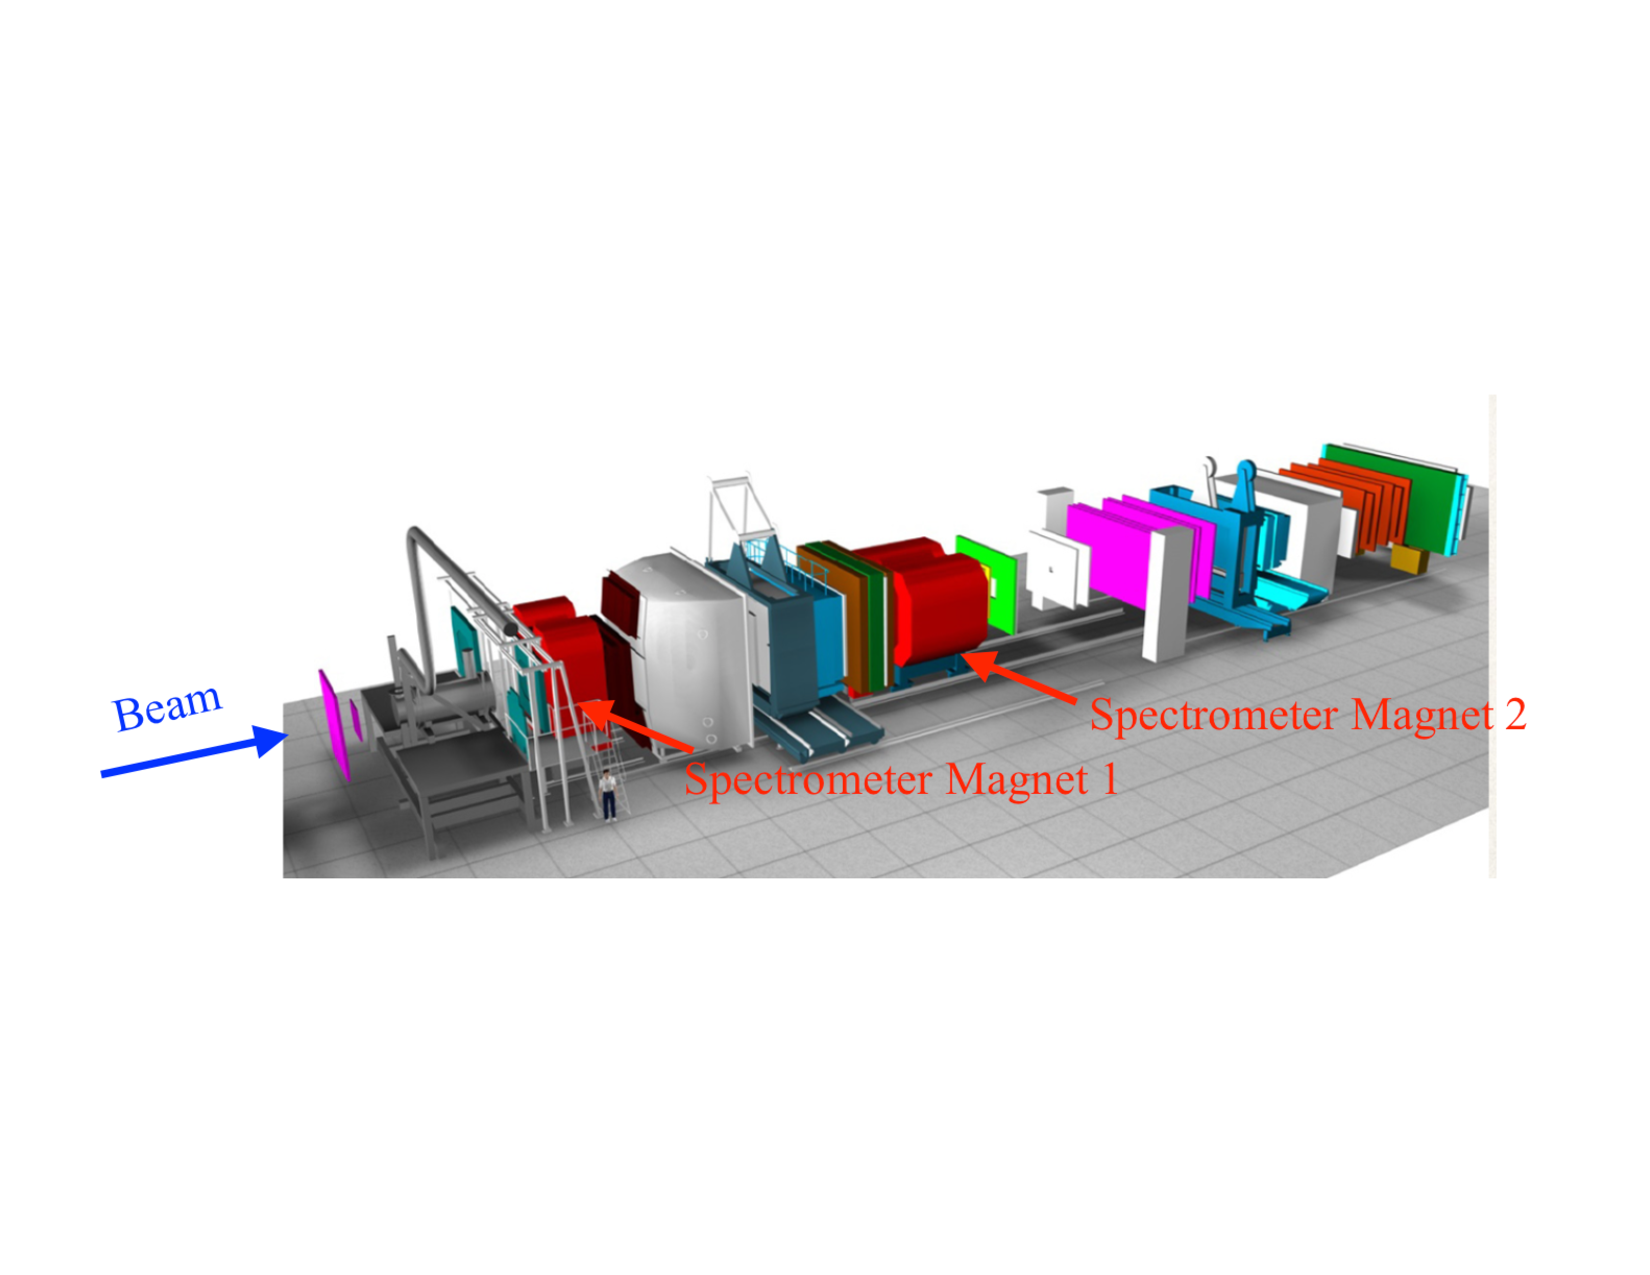
\includegraphics[width=\textwidth, trim=0.5cm 5cm 0.7cm 7cm,clip]{compassSpec}
  \caption{A schematic of the 2015 COMPASS setup}
  \label{fig::compassSpec}
\end{figure}

This chapter gives an overview of the COMPASS data taking setup with specific
interest on the 2015 setup from which the data in this thesis was produced from.
For a more thorough review of the spectrometer see
reference~\cite{compassSpec}.  This chapter is roughly organized by how the
data taking occurs.

\section{The Beam}
The COMPASS spectrometer receives beam from the Super Proton Synchrotron (SPS)
along on the M2 beam line.  A schematic of the M2 beam line is shown in
Fig.~\ref{fig::M2line}.  There are several different beam types and energies
available to COMPASS.  The most common types used for physics analysis are a
tertiary muon beam up to 190~{\gvc} and secondary hadron beam with an energy up
to 280~{\gvc}.  Both of these beam types can have a positive or negative charge.
As well it is possible to have a lower intensity tertiary electron beam which is
manly used for calibrations. \par

\begin{figure}[h!t]
  \centering
  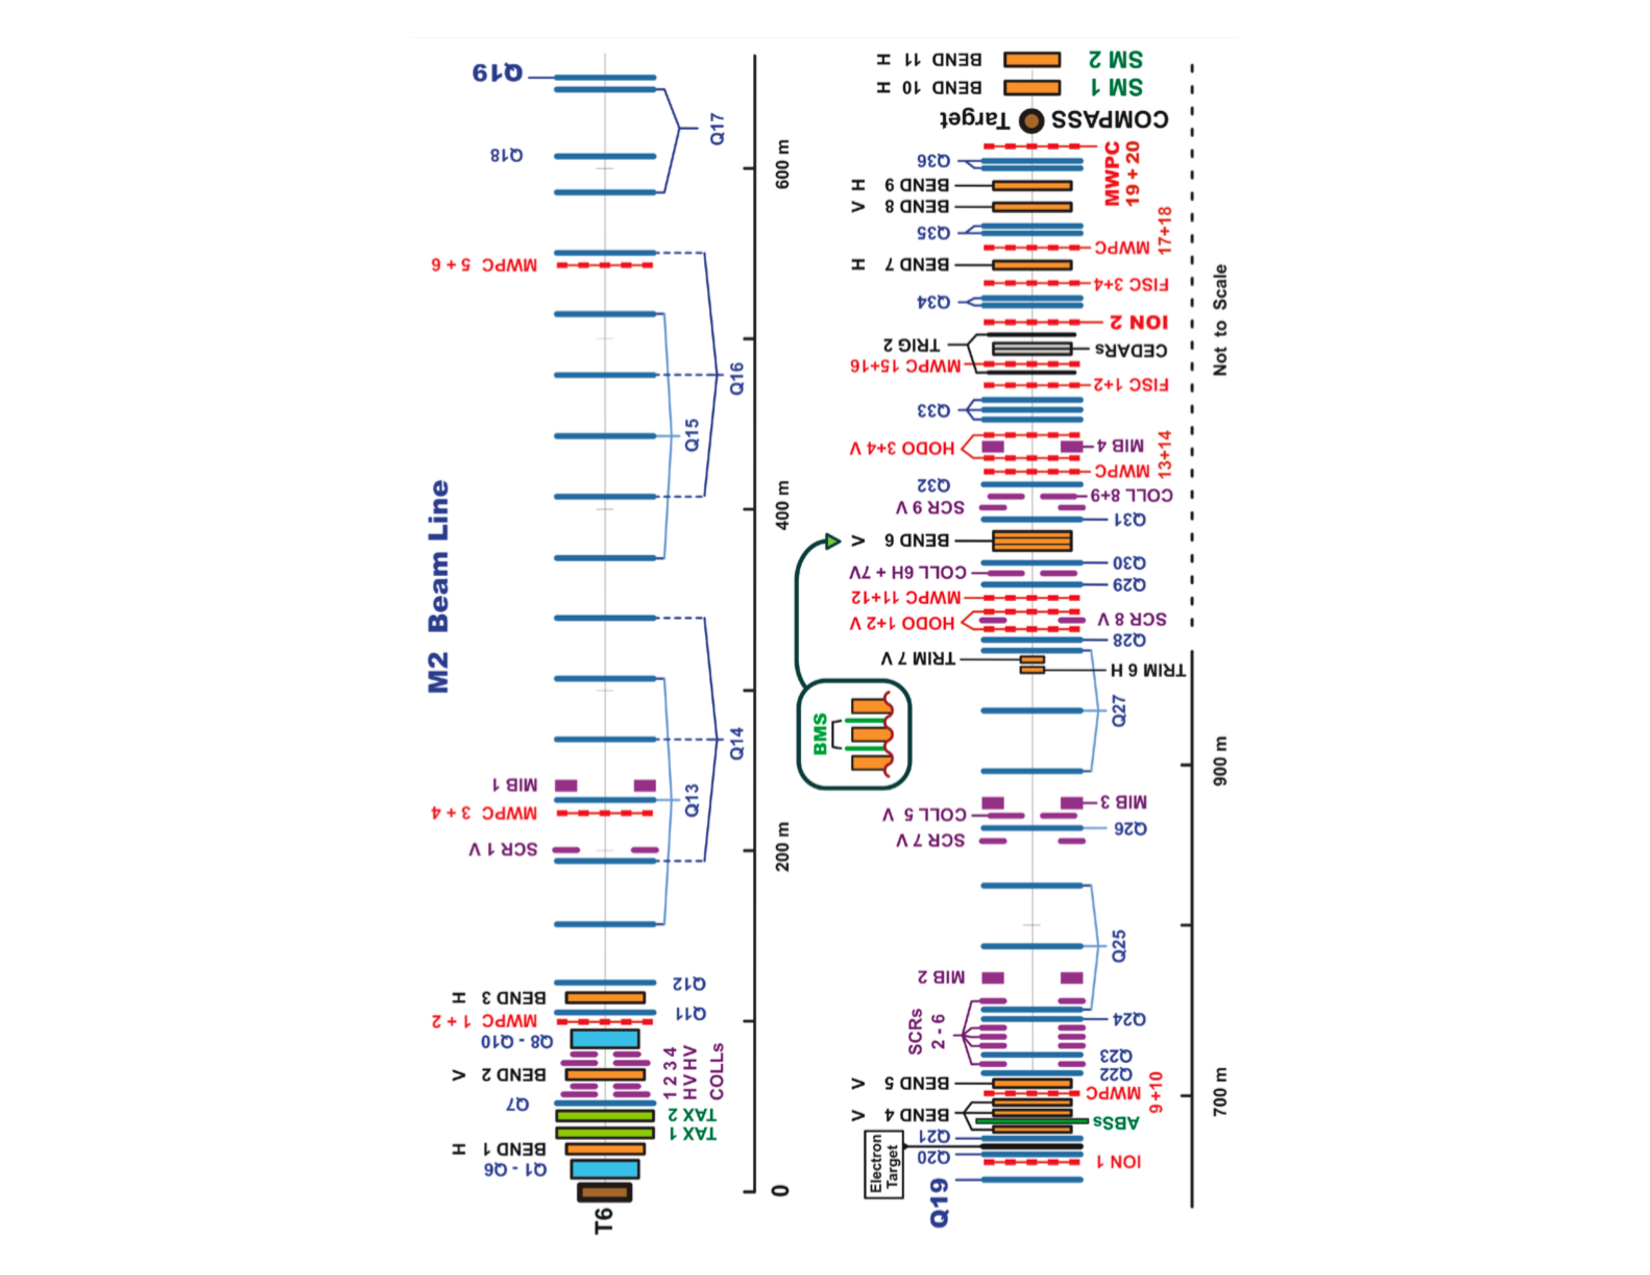
\includegraphics[width=\textwidth,trim=2cm 0cm 6cm 0cm,clip,angle=270]{M2line}
  \caption{The M2 beam line at CERN}
  \label{fig::M2line}
\end{figure}

The start of the M2 beam line is the T6 target which is made of beryllium and
has an adjustable length.  The SPS accelerates primary protons up to 400~{\gvc}
which impinges on the T6 target to produce a secondary beam.  The nominal proton
intensity on the T6 target is 100x10$^{11}$ spill$^-1$.  The longer the T6
target the higher the secondary intensity where 500mm is the longest and typical
target length used for physics data taking.  The reaction of the proton beam
with the T6 mainly produces secondary protons, pions and kaons.  Following this
reaction a series of dipole and quadruple magnets are used to select the
momentum and charge of interest. \par

The SPS spill structure varies throughout the data taking year depending mainly
on the needs of the Large Hadron Colider (LHC).  In 2015 the average intensity
provided was 0.6x10$^8$ s$^{-1}$ and the typical spill structure was two
4.8~second spills every 36~seconds.

\subsection{Muon Beam}
The muon beam is a tertiary beam which results from a weak decay of the
secondary beam.  After the initial proton reaction on T6 the resulting secondary
particles are momentum and charge selected and sent through a 600m tunnel with
focusing and de-focusing (FODO) quadruple magnets.  In this tunnel the pion and
kaons can decay as
\begin{equation}
  \pi^{-(+)} \rightarrow \mu^{-(+)} + \overline{\nu}_{\mu^-}(\nu_{\mu^+})
  \label{eqn::pionDecay}
\end{equation}
\noindent
and
\begin{equation}
  \kappa^{-(+)} \rightarrow \mu^{-(+)} + \overline{\nu}_{\mu^-}(\nu_{\mu^+}).
  \label{eqn::kaonDecay}
\end{equation}
\noindent
At the end of the tunnel a series of nine 1.1m long beryllium absorbers,
referred to as the ABS in Fig.~\ref{fig::M2line}, remove the remaining hadron
component of the beam which did not decay.  A 172~{\gvc} secondary beam is
chosen to achieve a 160~{\gvc} tertiary $\mu$ beam.  Due to the fact that the
neutrino in the reactions \ref{eqn::pionDecay} and \ref{eqn::kaonDecay} is
always left handed, the muon will be natural longitudinally polarized.  For the
muon momentum chosen the muon beam achieves a polarization of 80\%.

\subsection{Hadron Beam}
In the case of a hadron beam the ABS absorbers are not used and the decayed
muons are removed due to their lower momentum.  In the case of a negative hadron
beam the composition of the beam is approximately 97~\% $\pi^-$, 2.5\% kaons and
0.5\% $\overline{\mathrm{p}}$. The 2015 Drell-Yan data taking used a 190~{\gvc}
hadron beam. \par

After the decay tunnel the beam is bent upwards along another FODO tunnel of
length 250m before reaching the surface approximately 100m before the COMPASS
target.  A series of three dipole magnets, called bend 6, then bend the beam to
a horizontal position aimed at the COMPASS target.  Both upstream and downstream
of bend 6 are three tracking detectors (BM01-BM06) that make up the Beam
Momentum Station (BMS).  The BMS is the upstream most component of the COMPASS
spectrometer and is able to determine the beam momentum to better than 1\% of
the beam momentum with an efficiency of approximately 93\%.  Bend 6 and the BMS
are shown schematically in Fig.~\ref{fig::BeamLine1}. \par

\begin{figure}[h!t]
  \centering
  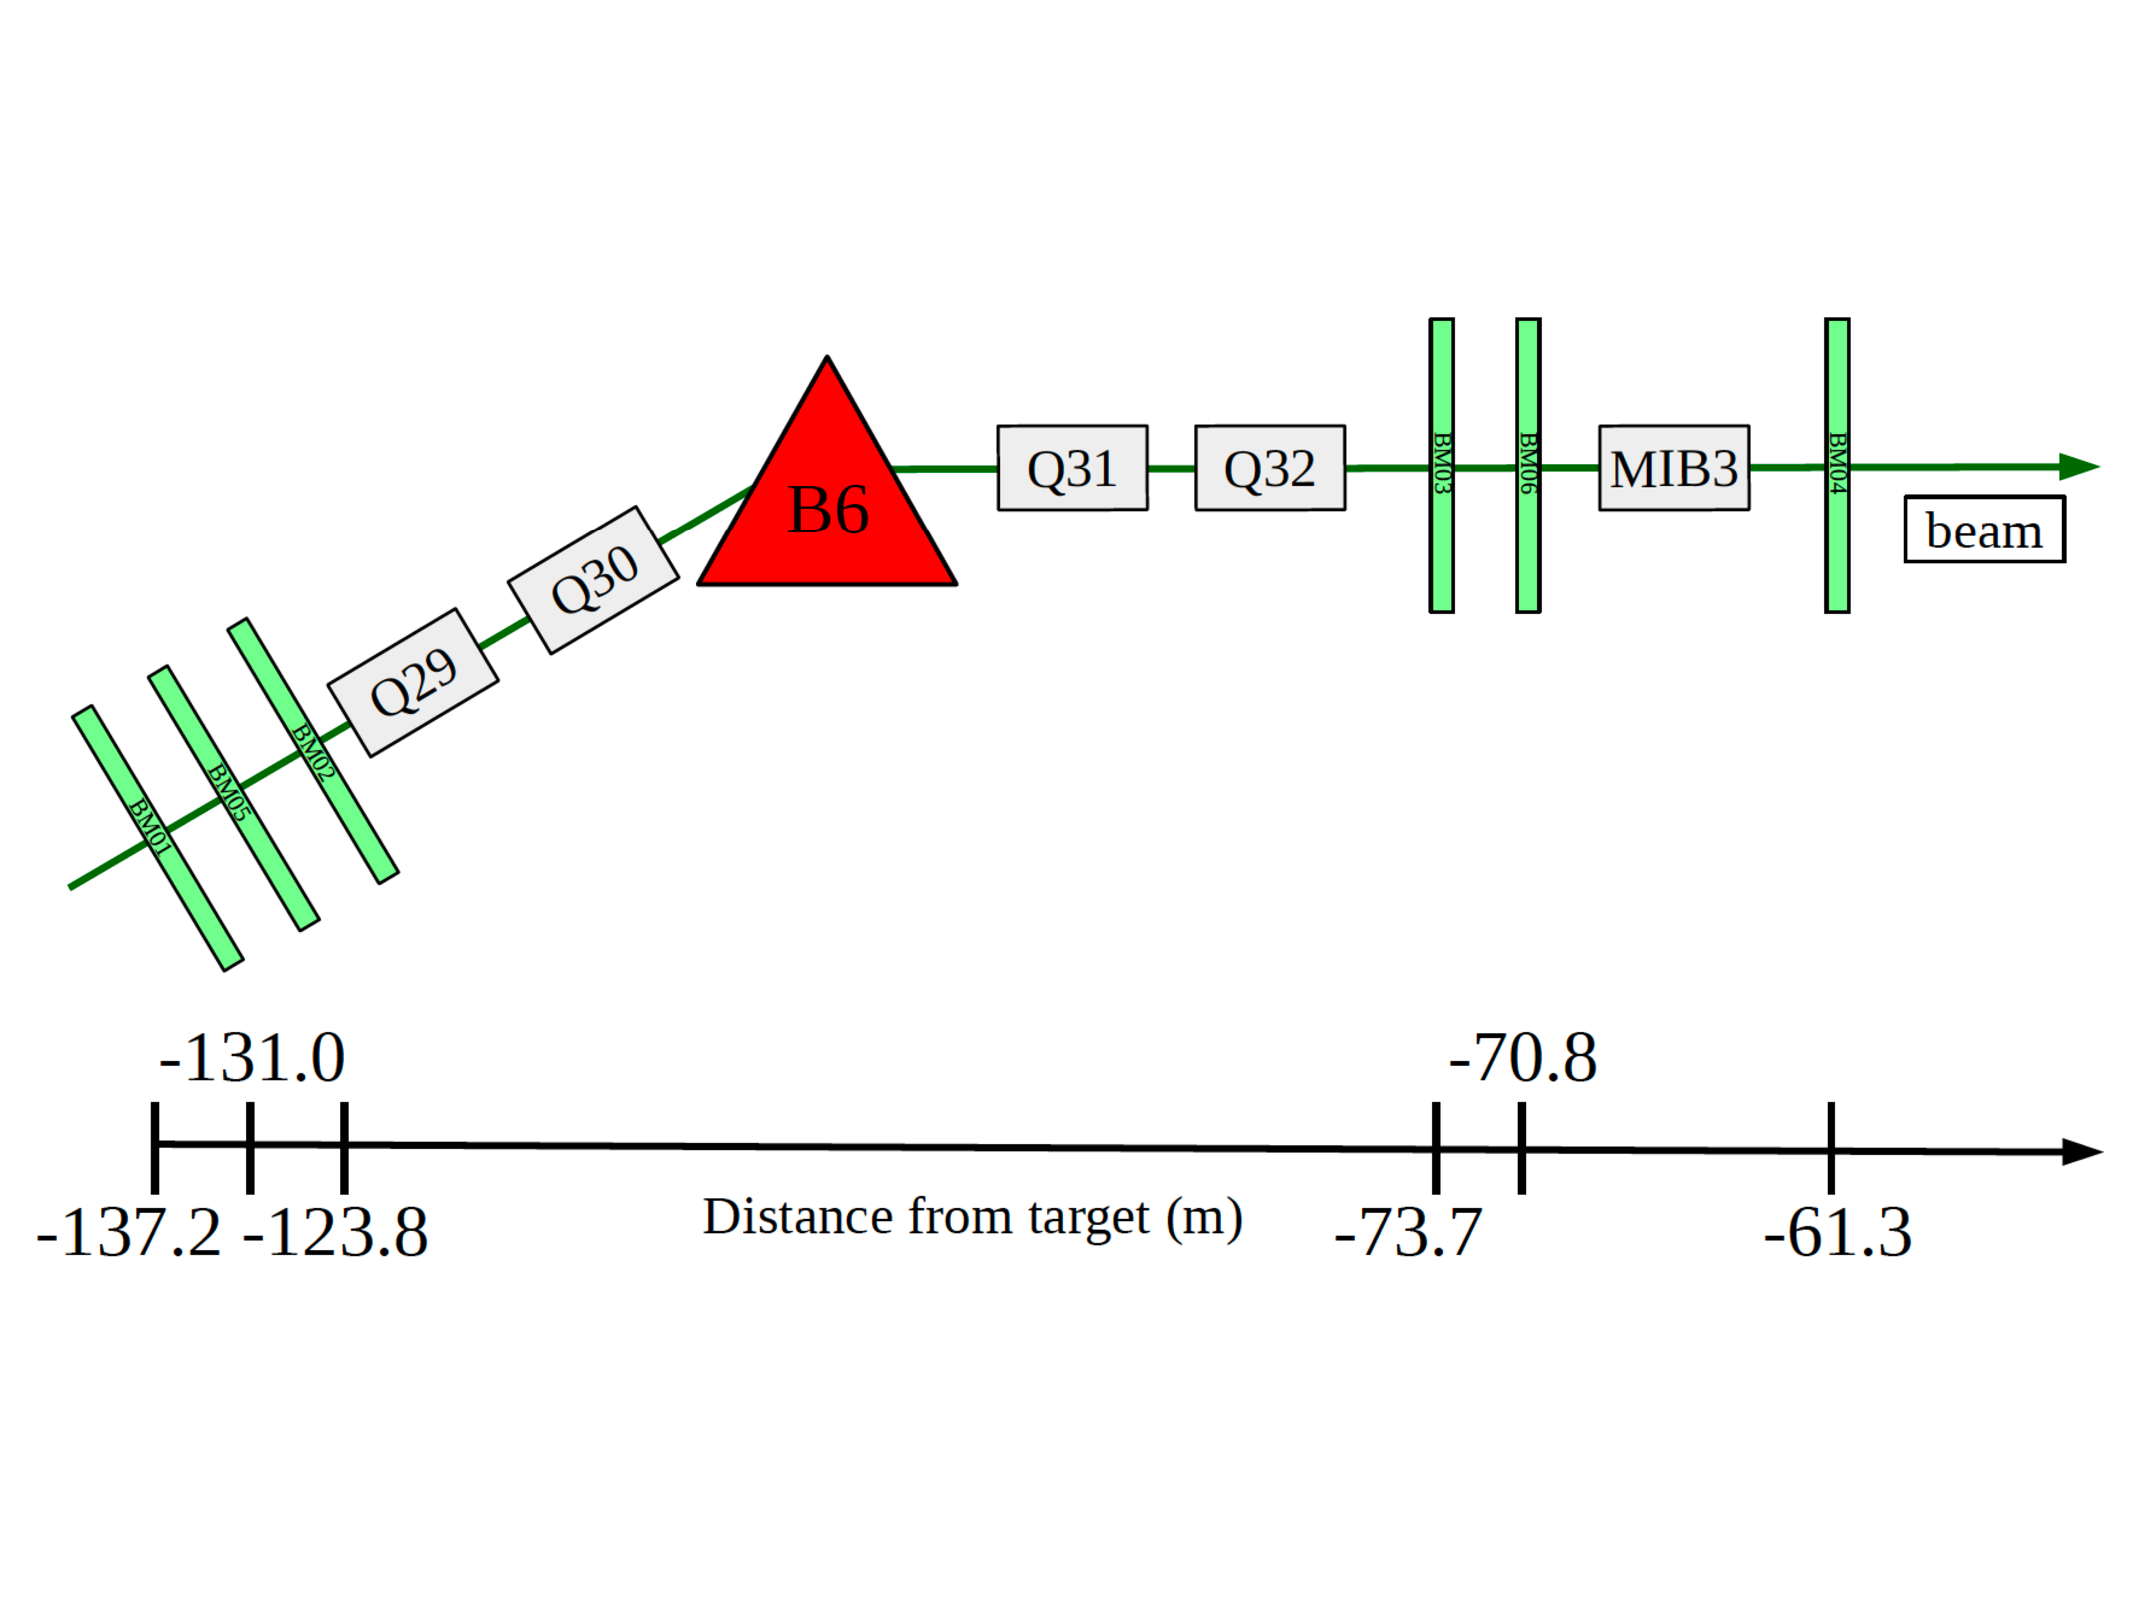
\includegraphics[width=0.8\textwidth]{BeamLine1}
  \caption{Bending the beam to a horizontal position.  The BMS detectors are
    upstream and downstream of the bend 6 magnet.}
  \label{fig::BeamLine1}
\end{figure}

For the 2015 Drell-Yan setup the $\pi^-$ beam intensity was too high for the BMS
station to work properly.  For this reason special low intensity, approximately
10$^6$ s$^{-1}$, $\pi^-$ beams were used in 2014 to determine the momentum
distribution for Drell-Yan data taking.  The beam momentum distribution is shown
in Fig.~\ref{fig::BeamMomBMS} where the average momentum is 190.9~{\gvc} with a
spread of $\pm$ 3.2~{\gvc}.

\begin{figure}[h!t]
  \centering
  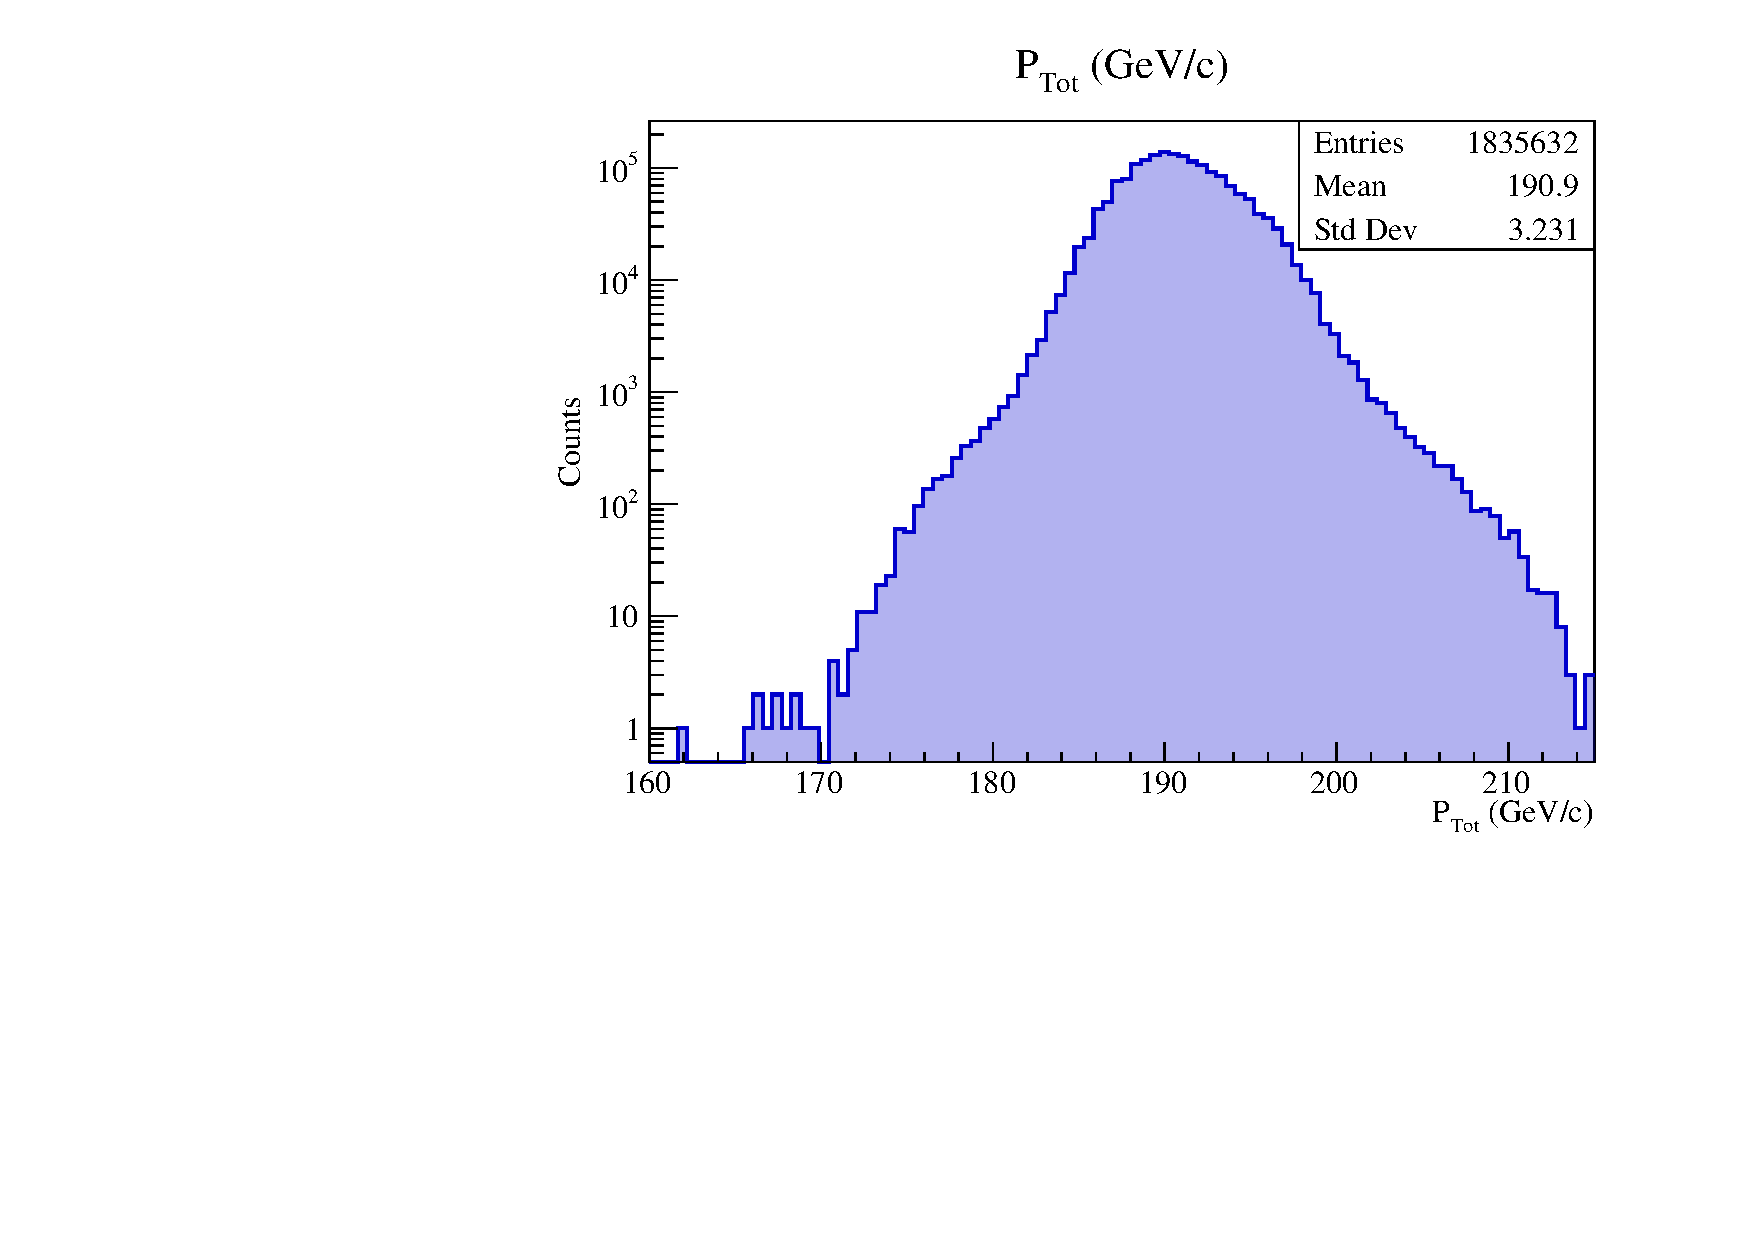
\includegraphics[width=0.6\textwidth]{BeamMomBMS}
  \caption{The momentum distribution of the $\pi^-$ beam, determined during
    dedicated low intensity beam times.}
  \label{fig::BeamMomBMS}
\end{figure}




\section{The Target}

\section{Tracking Detectors}

\section{Particle Identification}

\section{Trigger}

\section{Data Acquisition}

\section{Data Production}

\section{2015 Drell-Yan Setup}


This section of the spectrometer covers high
$Q^2$ and high $x_b$.  The target-pointing trigger system in LAS consists of two
hodoscopes, one down stream of the last tracker in LAS and the other just after
an iron muon filter in front of the second spectrometer magnet.

The trigger in SAS is
similar to the LAS trigger but for muons of a lower $Q^2$ value.  The tracking
detectors used in both spectrometers are gaseous detectors (drift chambers,
straws, multi-wire proportional detectors), micro-megas, and gas electron
multiplier (GEM) detectors.  The two stages are separated by two spectrometer
magnets: SM1, with a magnetic field integral of 1~Tm and SM2, with a magnetic
field integral of 4.4~Tm~\cite{compassSpec}.

Both SM1 and SM2 have magnetic
fields in the vertical direction meaning charged particles are deflected in the
x-z plane and can therefore have their momentum determined.  For beam
reconstruction there is a beam telescope upstream of the target consisting of
eight planes of scifi detectors.  To account for the transverse magnetic field
in the polarized target a chicane magnet system was added in the beam line.
This meant that the beam entered at a slight angle in the beam telescope but
exited the target going straight. \par

\section{The Beam old}
The Super Proton Synchrotron (SPS) is the second largest accelerator
at CERN.  It has a circumference of almost 7 km and it can accelerate
protons up to an energy of 450~GeV.  The SPS extracts beam to the
Large Hadron Collier and as well sends beam to various experiments in
the North Area at CERN.  COMPASS is one of these North Area
experiments, receiving beam tangent from the SPS on the M2 beam line.
In 2015 the SPS was delivering to COMPASS around $100 \times 10^{11}$
protons over a 4.9 second spill length and a spill was sent
approximately twice every 32 seconds.  The proton beam extracted from
the SPS then would collide with a primary 500~mm long, beryllium
target and from there a secondary hadron beam consisting of 97\% $\pi
^-$, 2\% $\bar{p}$ and 1\% $K^-$ was captured with magneto-optics into
a beamline leading to the COMPASS spectrometer.  The flux of the
secondary hadron beam averaged $0.6 \times 10^8
\frac{\mathrm{hadrons}}{\mathrm{sec}}$ and its momentum was
190~$\frac{\mathrm{GeV}}{\mathrm{c}}$~\cite{compassDYpaper}.



\section{Experimental Setup}

%\begin{figure}
%  \centering \includegraphics[width=0.3\textwidth]{Absorber}
%  \caption{The absorber at COMPASS was made of Alumina with a tungsten
%    plug and it was placed just downstream of the target cells.}
%  \label{fig::Absorber}
%\end{figure}





%\begin{figure}
%  \centering
%  %\includegraphics[width=\textwidth]{CompassSpectrometer}
%  \includegraphics[width=0.85\textwidth]{CompassSpectrometer}
%  \caption{The COMPASS spectrometer.}
%  \label{fig::COMPASS_spec}
%\end{figure}



The target material used was ammonia ($\mathrm{NH}_3$), where the proton from
the hydrogen nucleus was the polarizable nucleon.  The average polarization
throughout the data taking was 0.73 and a 0.6~T dipole magnet was used to
maintain target polarization.  With this dipole field and polarization, the spin
relaxation time for the target was approximately 1000 hours.  The target was
separated into two 55~cm cells of radius 2~cm which were in turn separated by
20~cm and oppositely polarized, as shown in figure~\ref{fig::Absorber}.  In 2015,
COMPASS took nine data periods labeled W07-W15.  Each data period lasted two
weeks and the spin orientation of the targets was reversed after the first week
of every period to reduce systematic effects arising from different geometric
acceptances and luminosities of up and downstream target cells.
%Most notably the spin
%orientation was reversed to have equal luminosity and to force equal
%geometrical acceptance between the two spin states. \par

%\begin{figure}[h]
%  \centering
%  \includegraphics[width=0.45\textwidth]{Absorber}
%  \caption{The absorber at COMPASS was made of Alumina with a tungsten
%    plug and it was placed just downstream of the target cells.}
%  \label{fig::Absorber}
%\end{figure}

For the 2015 Drell-Yan data taking a hadron absorber,
see figure~\ref{fig::Absorber}, was placed just downstream of the target
cells.  This was done to reduce the amount of hadrons and electrons
detected in the spectrometer and therefore ensured a cleaner di-muon
sample.  The absorber material was mostly alumina (Al$_2$O$_3$) and
concrete and the absorber corresponded to approximately 7.5
interactions lengths of material.  Inside the absorber was an aluminum
target followed by a tungsten plug, each of radius 2.5 cm, which acted
as a beam dump.  The aluminum target and tungsten plug served the
double purposes as absorbers and also as unpolarized nuclear targets.
In addition a thin $^6\mathrm{Li}$ absorber was added just downstream of the
primary absorber to absorb thermal neutrons produced in the primary
absorber.  This $^6\mathrm{Li}$ absorber was proposed to improve the
performance of the first tracking detector downstream of the
target. \par

\subsection{DAQ and Reconstruction}
The data acquisition system (DAQ) was recording events at a rate of
approximately 30~kHz with a dead time of 10\%.  In 2015, COMPASS
recorded approximately 750~terabytes of raw data from the nine,
two-week periods.  Raw data refers solely to individual detector
timing and wire or strip positions and does not correspond to physics
observables of interest.  From this raw information the CORAL
reconstruction software at COMPASS is able to determine the trajectory
and momentum of charged particles going through the COMPASS
spectrometer.

%This reconstruction stage reduces the data volume by approximately a factor of 10.
